\section{Implementering}

\subsection{Model}
Spillets model består af en række klasser, der tilsammen udgør selve spillets funktioner og objekter.

Klassen \textit{Field} bruges til at repræsentere et felt på banen. Den fungerer på samme måde som Javas standard \textit{Point}-klasse. Forskellen mellem \textit{Point} og \textit{Field}, er at vi bruger row og column i stedet for x og y. Spillepladen er delt op i rækker og kolonner, frem for en x- og y-akse. \textit{Field} er lidt mere selvdokumenterende og selve klasse navnet \textit{Point} giver ikke rigtig nogen indikation om hvad det point bruges til. Vores \textit{Field} har også den fordel at man ikke dynamisk kan ændre dens række og kolonne. De er låst fast til den samme værdi og kan kun ændres hvis man opretter et nyt \textit{Field} objekt.

Vi opretter en \textit{Food}-klasse som repræsentere et stykke mad på banen. \textit{Food} indeholder et \textit{Field} med madens position.

\textit{Food} og \textit{Field} har kun to værdier i sig (en række og søjle). Vi har designet klasserne sådan at de ikke kan ændres efter at de er blevet oprettet. Dette gør at vi kan returnere vores dem i getters og være 100\% sikre på at udefrakommende klasser ikke ændrer dem. Nogen gange kan det godt være svært at resonere omkring kode, hvis alle objekter vilkårligt kan ændre hinanden. Immutable klasser sikre at vi altid kan være sikker på at objekter ikke har ændret sig. Det gør at det er umuligt for Control-pakken at snyde spil logikken.

Slangen er defineret i \textit{Snake} klassen. Slangens krop består af en række felter, hvoraf det første er hovedet, og de resterende er kroppen inklusiv halen som er til sidst. Koordinaterne for disse felter er gemt som elementer i en ArrayList. Det første element er slangens første led, hovedet, det andet element er slangens andet led osv. Når slangen bevæger sig tilføjer vi et nyt hoved i listen og sletter halen. Hvis slangen bevæger sig og samtidig spiser noget \textit{Food}, so tilføjer vi kun et nyt hoved og lader være med at slette halen. Slangen vil altid være forholdsvis lille, så om vi gemmer dens elementer i for eksempel en ArrayList eller LinkedList er stort set lige meget. I \textit{Snake} konstruktøren bliver slangens hoved og hale oprettet. Hovedet bliver placeret i banens centrum. Halen placeres i kolonnen til højre for på samme hovedets række.

Vi har valgt at oprette spillepladen i \textit{Game}-klassen som et \textit{Dimension} objekt. Vi bruger ikke en \textit{Board}-klasse, der beskriver banen for sig selv. I bagklogskabens øje burde vi nok have brugt en \textit{Board} klasse. De andre spilelementer er defineret i deres egne klasser for eksempel \textit{Food} og \textit{Snake}.

Slangens \textit{move}-metoden flytter slangen. Den returnere et Action object, som en enum der betegner slangens handling. Om slangen spiser et æble, er død eller bevæger sig, henholdsvis \textit{EAT, KILL, MOVE}. I \textit{move}-metoden undersøges der, om der er mad på samme felt som hovedets nye placering. Er dette tilfældet, returneres \textit{EAT}. Hvis ikke, undersøges der om den nye placering for hovedet indeholder slangens krop. Gør der det returneres \textit{KILL}. Hvis ikke, flyttes slangens hoved til den nye position. Resten af slangens krop følger med ved at ændre koordinaterne i slangens ArrayList fra halen og op til hovedet.

I \textit{Game}-klassen findes \textit{checkAction}-metoden, der undersøger om slangen spiser eller dør. Hvis Action er \textit{EAT} inkrementeres scoren og der laves et nyt æble. Hvis Action-statementet er \textit{KILL}, nulstilles scoren, og spillet slutter ved at slangen ikke længere kan bevæge sig.

Herudover findes \textit{generateFood}-metoden, som sikrer, at maden altid placeres på et gyldigt felt, dvs. et felt der ikke er udfyldt af slangen. For at sikre dette, placeres æblet på et tilfældigt felt inden for banens rammer, hvorefter der undersøges om et af slangens led har samme koordinater som æblets felt. Er dette tilfældet, gives æblet et nyt felt, indtil det lander på et felt uden slangen. Er slangen tilpas stor, er dette dog ikke effektivt, da der er stor sandsynlighed for at ramme et felt, der er optaget af slangen. Af denne årsag undersøger metoden først, om slangen fylder mere end halvdelen af banen. Er dette tilfældet, laves der i stedet en liste med alle tomme felter vha. en for-løkke, der løber gennem alle række og kolonner, hvorefter et tilfældigt element i listen vælges som æblets position.

De fire klasser \textit{Food, Score, Game} og \textit{Snake} nedarver fra klassen \textit{Observable}, så det er muligt for View at modtage ændringerne i Model, uden at Control skal signalere til View at den har ændret Model.

\subsubsection{Immutable Model klasser}
Klasserne \textit{Food} og \textit{Field} er meget små. De har kun to værdier i sig (en række og søjle). Vi har designet klasserne sådan at de ikke kan ændres efter at de er blevet oprettet. Dette sikre os at vi kan returnere vores dem i getters og være 100\% sikre på at udefrakommende klasser ikke ændrer dem. Nogen gange kan det godt være svært at resonere omkring kode, hvis alle objekter vilkårligt kan ændre hinanden. Immutable klasser sikre at man altid kan være sikker på at objekter ikke har ændret sig. Det gør at det er umuligt for Control-pakken at snyde spil logikken.


\subsection{View (Brugergrænseflade)}
Brugerfladen er samlet i klassen \textit{GameView} der forlænger \textit{JFrame}. I \textit{GameView} findes kun en constructor, hvor der oprettes et \textit{ScorePanel}-objekt, der placeres øverst i vinduet, og et \textit{BoardPanel} objekt, der placeres direkte under det. Board-panelet viser selve banen med slangen og æblet, der begge er vist ved farvede firkanter. 

\textit{ScorePanel}-klassen forlænger \textit{JPanel} og implementerer \textit{Observer}. Klassen har en \textit{update}-metode, der gentegner, hver gang noget ændrer sig i de klasser i model-pakken, der forlænger \textit{Observable}. 
\textit{paintComponent}-metoden benyttes til at tegne score-teksten. Selve panelet oprettes i constructoren.

\textit{BoardPanel} forlænger også \textit{JPanel} og implementerer \textit{Observer}, for at den også kan registerere ændringer i model-klasserne. \textit{BoardPanel} består af en række draw-metoder, samt en \textit{paintComponent}-metode, der kalder på draw-metoderne for at tegne alle spillets komponenter på spillets bane og spillets bane selv.
I \textit{drawSnake}-metoden bruges positionerne for slangens felter til at tegne slangen. Størrelsen for et felt udregnes i \textit{getWindowRectangle}-metoden, og afhænger af vinduets størrelse og antallet af banens felter. Når feltets størrelse er udregnet, tegnes en rektangel med feltets størrelse på alle felterne i slangens positions-ArrayList.

Da spillepladen skal være mellem 5x5 og 100x100 felter, kan det skabe problemer, hvis man ikke kan justere størrelsen på vinduet. Vinduet kan være for stort til at passe på en gennemsnitlig computerskærm. Det er derfor nødvendigt at gøre spillets vinduestørrelse fleksibel. En løsning på dette problem ville være at bestemme en fast størrelse for felterne, og lade vinduet justere sin størrelse efter dette. Ulempen ved metoden er, at store baner kan blive for store til at være på en normal skærm. Derfor har vi valgt at lave en fleksibel størrelse for felterne, så de følger forholdet mellem vinduestørrelse og antal felter.
I figur \ref{fig:windowsize} kan man se, at hvis vinduet skal være justerbart, så kan man risikere at selve banen bliver aflang og ikke særlig pæn at spille på.

\begin{figure}[h]
	\centering
	\graphicspath{ {pics/} }
	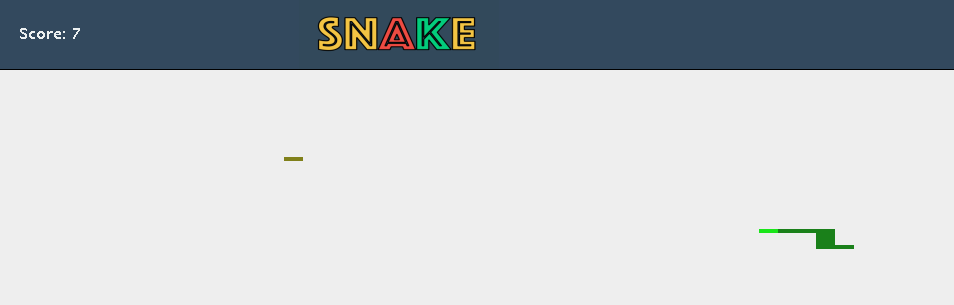
\includegraphics[width=0.8\textwidth]{WindowSize.png}
	\label{fig:windowsize}
	\caption{Exemple på udstræktede felter.}
\end{figure}

\subsection{Control (Styring)}
I Simpel Snake er der ikke brug for nogen menu, og det er derfor muligt at holde styringen af spillet meget simpelt. Ved at definere de fire piletaster i \textit{Control}-klassen, en funktion til at sikre at der ikke bevæges i modsat retning, samt en funktion der gør det muligt at bevæge sig som en torrus og "gå igennem vægge og om på den anden side af verden", er alle styringkrav til Simpel Snake opfyldt. Resten af spillet håndteres da i model-koden.

\textit{Control}-klassen har metoden \textit{keyPressed}, som kommer af at \textit{Control}-klassen implementerer \textit{KeyListener}, som kaldes hver gang der tastes på tastaturet. Hvis tasten er en af de fire piletaster, kaldes funktionen \textit{move} i \textit{Snake}-klassen, der flytter hovedet i samme retning som piletasten.
Enum-klassen \textit{Direction} indholder \textit{RIGHT, LEFT, UP} og \textit{DOWN}. Dette bruges i \textit{Control}-klassen, da det ikke skal være muligt at bevæge sig i modsatte retning af slangens nuværende retning.
I \textit{Control}-klassens constructor er Direction som udgangspunkt sat til \textit{LEFT}, da slangen starter mod venstre. Hver gang der tastes på piletasterne, sikrer \textit{keyPressed}-metoden, at retningen ikke er modsat af den nuværende retning. Herefter flyttes slangen, uanset om den er midt på spillepladen eller om den bevæger sig rundt om torussen. Til sidst sættes \textit{Direction} til den nuværende retning, så det ved næste tasteanslag igen kan undersøges, at retningen ikke er modsat.
